\chapter{Installation}
\label{chapter:Installation}

\index{Installation|textbf}

This section describes the process for installing ITK in your system. Keep in
mind that ITK is a toolkit library, as such, once it is installed in your
computer there will be no executable to run. The system provides a large set
of test files and examples that will help you to get introduced to the
concepts of ITK and will show you how to use ITK in your own projects.

Some of the examples distributed with ITK require third party libraries that
you may have to download. For a first installation of ITK you may want to
ignore these extra libraries and just built the toolkit itself. A large
fraction of the traffic on the users-mailing list originates from
difficulties in getting third party libraries installed rather than on actual
problems building ITK.

ITK has been developed and tested over multiple platforms including
MS-Windows, Linux, Solaris, IRIX and recently the Mac. Popular compilers like
Visual Studio 6.0, Visual Studio 7.0, gcc 2.95.2, gcc 2.96, gcc 3.04, gcc
3.1, gcc 3.2, Borland 5.5 and SGI-CC 6.5 are currently supported. Given the
extensive use of state of the art C++ in the toolkit some compiler may have
difficulties building the code. If you are currently using an outdated
compiler here may be an excellent excuse for upgrading this old piece of
software!

\section{Downloading ITK}
\label{sec:DownloadingITK}
 
\index{Downloading|textbf}

ITK can be downloaded free of charge from the following web site:
\begin{center} 
  \url{http://www.itk.org}
\end{center}
In order to track the kind of applications for which ITK is being used, you
will be kindly asked to fill a form before downloading the software.
The information you provide in this form will help developers to get a better
idea of the interests and skills of the toolkit users. 

Once you fill this form you will have access to the download page where two
options for downloading the software will be found. This page can be bookmarked
to facilitate a second visit to the download site without having to fill any
form again. You can get the tarball of a stable release or you can get the
development version through CVS.  The release version is stable and dependable
but may lack the latest features of the toolkit. The CVS version will have the
latest additions but is inherently unstable and may contain components with
work in progress.  The following sections describe the details of each one of
these two alternatives.

\subsection{Downloading the tarball}
\label{sec:DownloadingTarballs}

\index{Downloading!tarballs}

Please read the \code{GettingStarted.txt}
\footnote{http://www.itk.org/HTML/GettingStarted.txt} document first. It will
give you an overview of the download and installation processes. Then choose
the tarball that better fits your system. The options are .zip and .tgz files.
The first type is better suited for MS-Windows while the second one is the
preferred format for UNIX systems.

Once you unzip or untar the file a directory called \code{Insight} will be
created in your disk and you will be ready for starting the configuration
process described in section \ref{sec:CMakeforITK}.

\subsection{Downloading from CVS}
\label{sec:DownloadingFromCVS}

\index{Downloading!CVS repository}
\index{CVS!downloading from}

The Concurrent Versions System (CVS) is a tool for version control
\cite{Fogel1999}. It is a very valuable resource for Open Source projects
involving multiple developers.  CVS maintains a code repository with the
multiple versions of every source code file in the project. Developers can
check out code to their local systems, modify the code and commit the
modifications to the central repository. CVS will take care of merging
modifications and notify about potential conflicts.  It also maintains the
whole history of the project.

Developers and users can check out the software from the CVS repository. When
developers introduce changes in the system,  CVS facilitates to update the
local copies of other developers and users by downloading only the differences
between their local copy and the version on the repository.  This is an
important advantage for those who are interested in keeping up to date with the
leading edge of the toolkit. Bug fixes can be obtained in this way as soon as
they have been checked into the system.

The CVS version of ITK contains the current state of the project. Since ITK
is under active development the current version is not necessarily stable. If
you decide to use this version it is important that you take a look at the
on-line quality control dashboard first. The Dashboard indicates how the
current version is being compiled and tested in a variety of platforms (see
section \ref{sec:QualityDashboard} for details).

You will need to have CVS installed in your system. This is quite standard on
UNIX systems, typing \code{cvs -version} on the command line should be enough
to verify that cvs is installed. You will need CVS version 1.11 to download
ITK.  On MS-Windows systems you have two options for using CVS. The first one
is to install \code{Cygwin} which is the equivalent of having a UNIX
installation on top of Windows. Cygwin will provide most (if not all) of the
current packages and utilities available in UNIX systems, including
CVS. Cygwin can be downloaded for free from
\url{http://www.redhat.com}. The second option is to use \code{WinCVS} 
which is a Windows native applications that provides a standard graphic user 
interface to CVS. WinCVS can be downloaded for free from 
\url{http://www.wincvs.org/}.

Once you find that the current state of the toolkit is stable you can download
ITK by using the following commands (under UNIX and Cygwin): 
\begin{verbatim}
cvs -d :pserver:anonymous@www.itk.org:/cvsroot/Insight login
(respond with password "insight")

cvs -d :pserver:anonymous@www.itk.org:/cvsroot/Insight co Insight
\end{verbatim}

This should trigger the download of the software into a directory named
\code{Insight}.  Any time you want to update your version, it will be enough to
move inside this directory and to type 
\begin{verbatim}
cvs update -d -P
\end{verbatim}

Now you are ready to follow the configuration instructions described in section
\ref{sec:CMakeforITK}.

\subsection{Joinning the Mail List}
\label{sec:JoinningMailList}

\index{Mailing list|textbf}

It is strongly recommended that you join the users mailing list. This is one
of the primary resources to get guidance and orientation about the use of the 
toolkit. You can subscribe to the users list on-line at
\begin{center}
\url{http://www.itk.org/HTML/MailingLists.htm}
\end{center} 

The insight-users mailing list is also the best mechanism for expressing your
opinions about the toolkit and let developers know about the features that
you find useful, desirable or eventually unnecessary in the toolkit. ITK
developers are committed to construct a self-sustained Open Source
community. Feedback from users is fundamental to achieve this goal.

\subsection{The Quality Dashboard}
\label{sec:QualityDashboard}

\index{Dashboard|textbf}
\index{Quality Dashboard|textbf}
\index{Dart|textbf}

Quality Control is an important component of Open Source projects. It allows
to keep the evolution of a project under control by detecting inconsistencies
and errors early on when they are introduced in the system. ITK uses the Dart
system for quality control.
 
\begin{figure}[ht]
\centering 
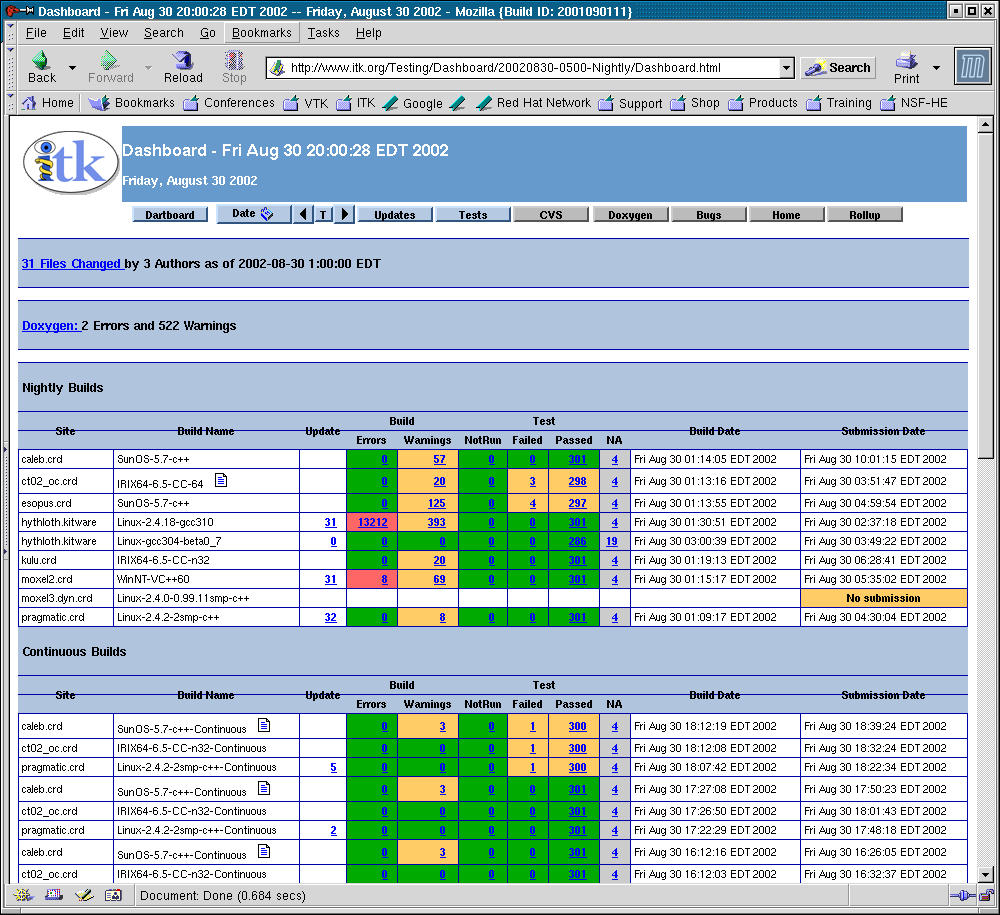
\includegraphics[width=0.7\textwidth]{Dashboard.eps}
\caption{On-line presentation of the Quality Dashboard generated by Dart}
\label{fig:Dashboard}
\end{figure}

Dart administers a Web site where the results of compiling the toolkit are
submitted by multiple machines. ITK contains and extensive set of testing
files that exercise all the classes and their methods.  The continuous
compilation of these testing files acts as an early warning mechanism to spot
the introduction of errors on the toolkit. Because the Dart dashboard can be
seen on-line, developers and users can monitor the current state of the
system and rapidly track problems down to their source.  Tracing history of
every test is also possible from this web site.

The ITK Dashboard can be found on-line at
\begin{center} 
\url{http://www.itk.org/Testing/Dashboard/MostRecentResults-Nightly/Dashboard.html}
\end{center} 

Figure \ref{fig:Dashboard} shows the Dashboard HTML page. Each row in the
Dashboard corresponds to a particular platforms (hardware + operating system
+ compiler). The data on the row indicates the number of compile errors and
warnings as well as the results of the execution of hundreds of small test
programs. In this way the toolkit is tested both at compile time and run
time.

When users decide to download the CVS version of ITK it is important for them
to verify first that the current dashboard is in good shape. This can be
rapidly judged by the general coloration of the Dashboard. A green state
means that the software is building correctly and it is a good day to start
with ITK or to get an upgrade. A red state, on the other hand, is an
indication of instability on the system and hence users should better refrain
from checking out or updrading. Red states are usually cleared the same day.

Dart is independent of ITK and can be used for supporting quality control of
any software project. It is itself an Open Source package and can be
downloaded from

\begin{center} 
\url{http://public.kitware.com/Dart/HTML/Index.shtml}
\end{center} 

\section{Configuring ITK}
\label{sec:ConfiguringITK}

\index{Configuration|textbf}
 
The challenge of making ITK multi-platform led early on in the project to
address the problem of configuring the toolkit for different systems. The
response to this challenge was the development of CMake, a cross-platform,
open-source make system. CMake is used to control the software compilation
process using simple platform and compiler independent configuration files.
CMake generates native makefiles and workspaces that can be used in the
compiler environment of your choice. CMake is quite sophisticated, it makes
possible to support complex environments requiring system configuration,
pre-processor generation, code generation, and template instantiation.

CMake generates Makefiles under UNIX and Cygwin systems and generates Visual
Studio workspaces under Windows. The information used by CMake is provided by
files named \code{CMakeList.txt} which have been created on every directory
of the ITK source tree. This information is complemented with parameters that
the user should provide to CMake at configuration time. Typical information
provided by the user includes paths to utilities in the system and selection
of options that are associated to user's preferences.

\subsection{Preparing CMake}
\label{sec:CMakeforITK}
 
\index{CMake|textbf}
\index{CMake!downloading}

CMake can be downloaded for free from 
\begin{center} 
  \url{http://www.cmake.org}
\end{center}

ITK require the latest release of CMake\footnote{The current version at the
time of writing this document is CMake 1.4 patch 7}. You can download binary
versions for most of the popular platforms including Windows, Solaris, IRIX,
HP, Mac and Linux. You can alternatively download the code and build CMake by
yourself on your system. It is very important to avoid to have several
different versions of CMake simultaneously. The reason is that CMake searches
you system in order to find its components, and mixing components from
different version will produce inconsistent executables. Follow the
instructions in the CMake web page for downloading and installing the system.

Once CMake is built you will run its executable and provide the directory
where resides the source code to be configured and the directory where the
compiled binary code should be stored. The selection of this last directory
is at your will according to your preferences for organizing your disk.

CMake will run in an interactive mode in which you will progresively select
options and configure according to these options. At each configuration
iteration, CMake will evaluate if whether new options have to be presented to
the user or not. This can be better understood if you imagine that you are
walking through a decision tree.  Every option that you select may open the
possibility for further options to become relevant. When this is the case,
the new options will be presented by CMake at the top of the options list in
its interface.  Only when no new options appear after a configuration step
you will be sure that the necessary decisions have all been made and that you
are ready for generating the Makefiles or Visual Studio project for the
current configuration.

\subsection{Configuring ITK}
\label{sec:ConfiguringITKwithVTK}
  
\index{Configuration!with VTK}

\begin{figure}[ht]
\centering 
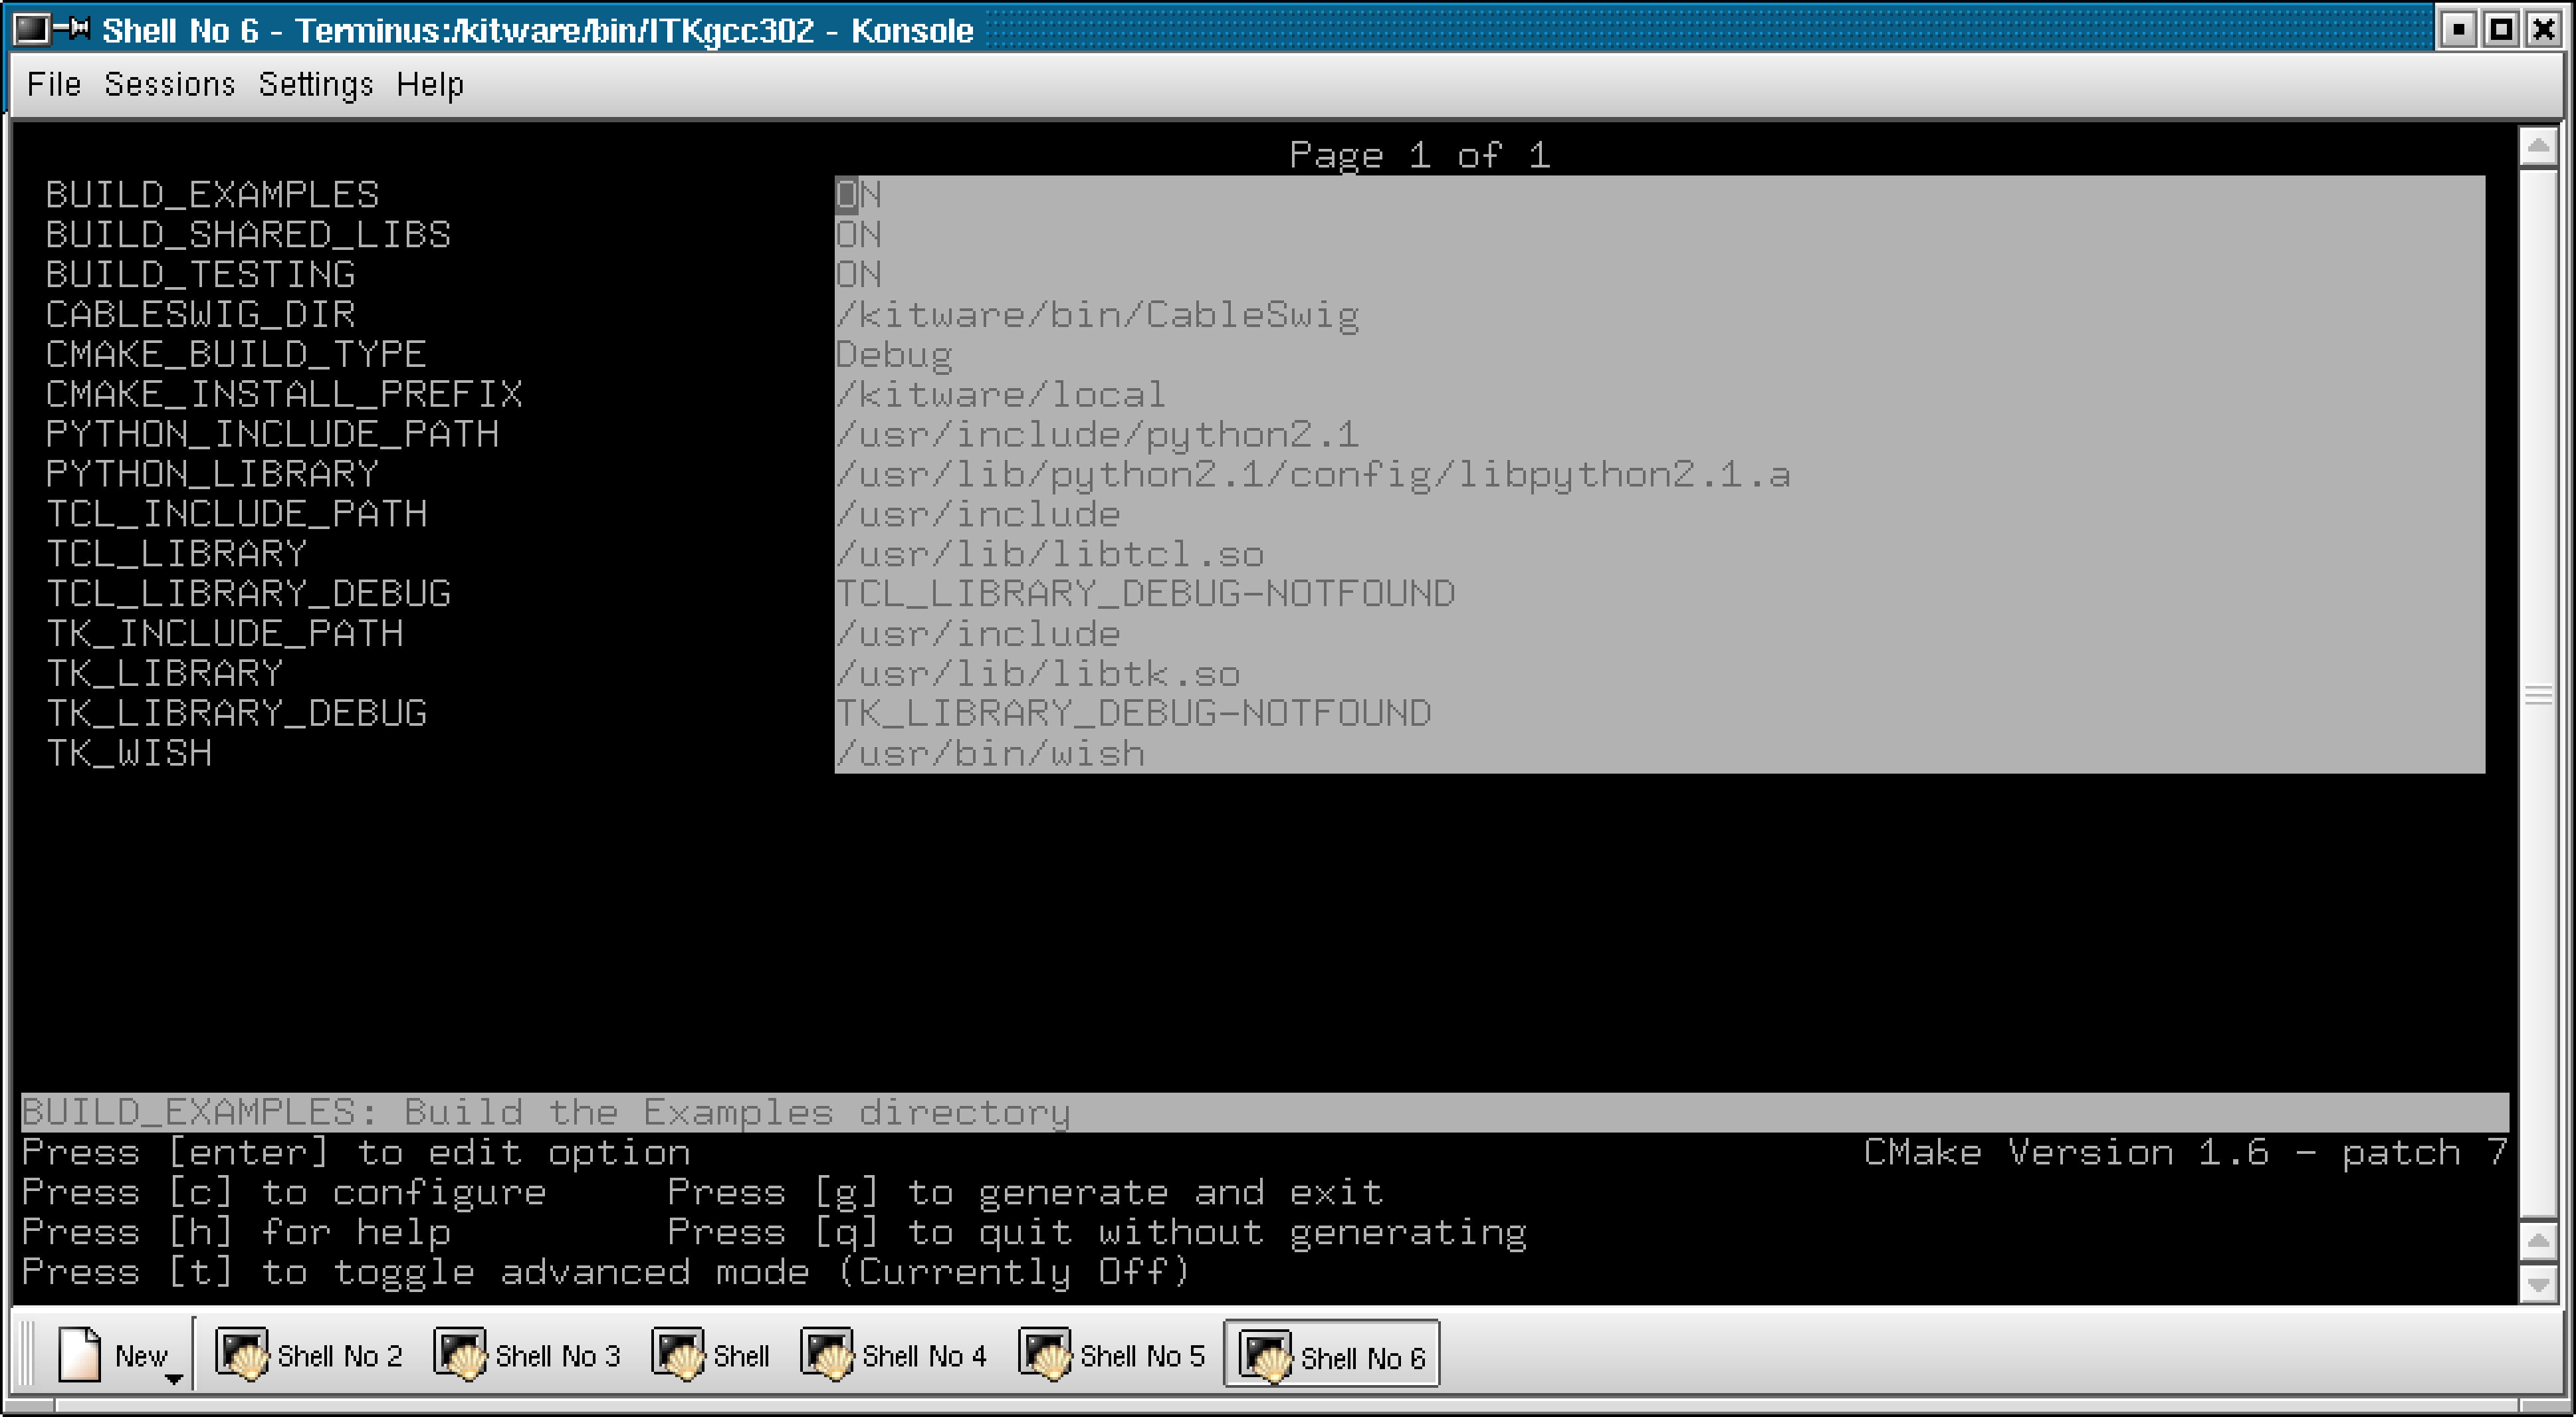
\includegraphics[height=0.45\textwidth]{ccmakeScreenShot.eps}
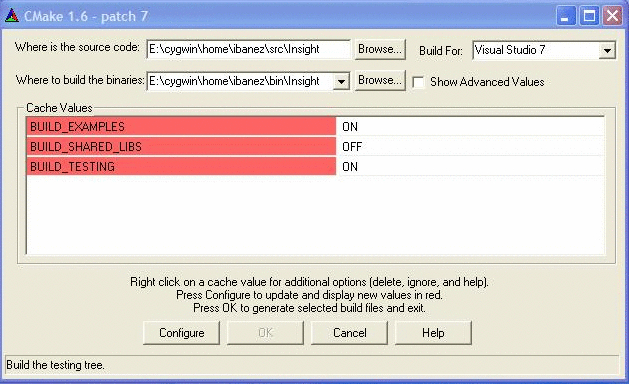
\includegraphics[height=0.45\textwidth]{CMakeSetupScreenShot.eps}
\caption{CMake interface. Left) \texttt{ccmake}, the UNIX version based on
\texttt{curses}. Right) \texttt{CMakeSetup}, the MS-Windows version based on MFC}
\label{fig:CMakeGUI}
\end{figure}

Figure \ref{fig:CMakeGUI} shows the CMake interface for UNIX and MS-Windows.
In order to speed up the build process you may want to disable the
compilation of the demo applications. This is done with the variable
\code{BUILD\_APPLICATIONS=OFF}. The demo applications  distributed with the
toolkit are a helpful resource for learning how to write problem-oriented
applications.  However, due to the large number of examples and the fact that
some of them rely on third party libraries that need to be installed and
configured, enabling this option will considerably complicate the initial
configuration of the toolkit.

Each time you change a set of variables in CMake, it is necessary to proceed
to another configuration step. In the Windows version this is done by
clicking on the ''Configure'' button. In the UNIX version this is done in a
\code{curses} interface where you can select to configure by hitting the
''c'' key.

When no new options appear in CMake, you can proceed to generate Makefiles or
Visual Studio projects. This is done in Windows by clicking on the ''Ok''
button.  In the UNIX version this is done by hitting the ''g'' key. After the
generation process is done CMake will quit silently. To initate the build
process, you can under UNIX simply type \code{make} while under Window you
will have to load the workspace named \code{ITK.dsw} from the directory that
you provide to CMake as Binary directory.

The build process will typically take from 30 minutes to one hour depending
on the performance of your system. As part of the normal built process, about
300 small test programs are compiled. This allows to verify that the basic
components of ITK have been correctly built on your system.

\section{Using ITK }
\label{sec:UsingITK}
 
The simplest way to get started with ITK is to create a new directory
somewhere in your disk and write two files on it. The first one is a
\code{CMakeList.txt} file which will be used by CMake to generate a Makefile
(if you are using UNIX) or a Visual Studio workspace (if you are using
MS-Windows).  The second file is an actual C++ file that will exercise some of
the multiple classes available in ITK.

Once both files are in your directory you can run CMake in order to configure
your project. Under UNIX, you can \code{cd} to your newly created directory
and type \code{"ccmake . "}. Note the "." in the command line for indicating
that the \code{CMakeList.txt} file is in the current directory. The
\code{curses} interface will require you to provide the directory where ITK
was built. This is the same path that you indicated for the
\code{ITK\_BINARY\_DIR} variable at the time of configuring ITK. Under
Windows you can run \code{CMakeSetup} and provide your newly created
directory as being both the source directory and the binary directory for
your new project. In CMake jargon this is called an
\emph{in-source} built. Then CMake will require you to provide the path to the
binary directory where ITK was built. The ITK binary directory should contain a
file named \code{UseITK.cmake} that was generated during the configuration
process at the time ITK was built.  From this file CMake will efficiently
recover all the information required to configure your new ITK project.  

\subsection{Hello World !}
\label{sec:HelloWorldITK}

\index{Hello World|textbf}

Here is the content of the two files to write in your new project. First, the
\code{CMakeList.txt} file.

\begin{verbatim}
PROJECT(mySampleProject)

INCLUDE (${CMAKE_ROOT}/Modules/FindITK.cmake)
IF (USE_ITK_FILE)
  INCLUDE(${USE_ITK_FILE})
ENDIF(USE_ITK_FILE)

LINK_LIBRARIES( ITKCommon )
ADD_EXECUTABLE(SampleProject SampleProject.cxx )
\end{verbatim}

The first line will define the name of your project as it appears in Visual
Studio (it will have no effect under UNIX). The second line loads a CMake
file with a predefined strategy for finding ITK \footnote{Similar files are
provided in CMake for other commonly used libraries, all of them named
\code{Find*.cmake}}. If the strategy for finding ITK fails, CMake will prompt
you for the directory where ITK is installed in your system. In that case you
will write This information in the \code{ITK\_DIR} variable. The line \code{
INCLUDE(\${USE\_ITK\_FILE})} loads the UseITK.cmake file containing all the
configuration information from ITK. The \code{LINK\_LIBRARIES} line specify
which ITK libraries will be linked against this project. Finally the line
\code{ADD\_EXECUTABLE} defines as its first argument the name of the executable
that will be produced as result of this project. The following arguments in the
line are the names of the source files to be compiled and linked.

The source file \code{SampleProject.cxx} should have the following content

\begin{verbatim}
#include "itkImage.h"
#include <iostream>
int main() 
{
  typedef itk::Image< char, 3 > ImageType;
  ImageType::Pointer image = ImageType::New();
  std::cout << "ITK Hello World !" << std::endl;
  return 0;
}
\end{verbatim}

This declares a 3D image \footnote{also known as a volume} whose pixels are
of type \code{char}.  The Image class is explained in detail in section
\ref{sec:ImageSection}.



